\documentclass[journal,12pt,twocolumn]{IEEEtran}
\usepackage{cite}
\usepackage{amsmath,amssymb,amsfonts,amsthm}
\usepackage{algorithmic}
\usepackage{graphicx}
\usepackage{textcomp}
\usepackage{xcolor}
\usepackage{txfonts}
\usepackage{listings}
\usepackage{enumitem}
\usepackage{mathtools}
\usepackage{gensymb}
\usepackage{comment}
\usepackage[breaklinks=true]{hyperref}
\usepackage{tkz-euclide}
\usepackage{listings}
\usepackage{gvv}
\def\inputGnumericTable{}
\usepackage[latin1]{inputenc}
\usepackage{color}
\usepackage{array}
\usepackage{longtable}
\usepackage{calc}
\usepackage{multirow}
\usepackage{hhline}
\usepackage{ifthen}
\usepackage{lscape}
\usepackage{circuitikz}
\usepackage{geometry}

\newtheorem{theorem}{Theorem}[section]
\newtheorem{problem}{Problem}
\newtheorem{proposition}{Proposition}[section]
\newtheorem{lemma}{Lemma}[section]
\newtheorem{corollary}[theorem]{Corollary}
\newtheorem{example}{Example}[section]
\newtheorem{definition}[problem]{Definition}
\newcommand{\BEQA}{\begin{eqnarray}}
\newcommand{\EEQA}{\end{eqnarray}}
\newcommand{\define}{\stackrel{\triangle}{=}}
\theoremstyle{remark}
\newtheorem{rem}{Remark}

\begin{document}

\bibliographystyle{IEEEtran}
\vspace{3cm}

\title{Gate 2021- EC}
\author{EE23BTECH11058 - Sindam Ananya$^{*}$% <-this % stops a space
}
\maketitle
\newpage
\bigskip

\renewcommand{\thefigure}{\theenumi}
\renewcommand{\thetable}{\theenumi}

\vspace{3cm}
\textbf{Question 4:} 
Consider a real-valued base-band signal $x(t)$, band limited to $10kHz$. The Nyquist rate for the signal \\\\
$y(t) = x(t)x(1+\dfrac{t}{2})$ is\\

\begin{enumerate}
\item[(A)] $15kHz$
\item[(B)] $30kHz$
\item[(C)] $60kHz$
\item[(D)] $20kHz$
\end{enumerate}
\hfill{(GATE EC 2021)}\\
\solution
\begin{table}[h!]
\centering
\begin{tabular}{|c|c|c|}
\hline
\textbf{Parameter} & \textbf{Value} & \textbf{Description}\\
\hline
$x(t)$ & & base-band signal\\
\hline
$f$ & $10kHz$ & Maximum frequency of $X(f)$\\
\hline
$y(t)$ & $x(t)x(1+\dfrac{t}{2})$ & new signal\\
\hline
$f_{max}$ & & Maximum frequency of $Y(f)$\\
\hline
\end{tabular}

\caption{Input Parameters}
\label{tab:gate2021ec4table}
\end{table}
\begin{align}
x(t) &\xleftrightarrow{\mathcal{F}} X(j\omega)\\
x(at) &\xleftrightarrow{\mathcal{F}} \frac{1}{a}X(j\omega)\\
x(t-t_o) &\xleftrightarrow{\mathcal{F}} e^{-j\omega t_o}X(j\omega)\\
x(1+\frac{t}{2}) &\xleftrightarrow{\mathcal{F}} 2e^{j\omega}X(j2\omega)\\
y(t) &= x(t)x(1+\frac{t}{2})\\
x_1(t)x_2(t) &\xleftrightarrow{\mathcal{F}} X_1(f) * X_2(f)\\
Y(f) &= X(f) * 2e^{j2\pi f}X(2f)
\end{align}
\begin{figure}[h!]
    \centering
    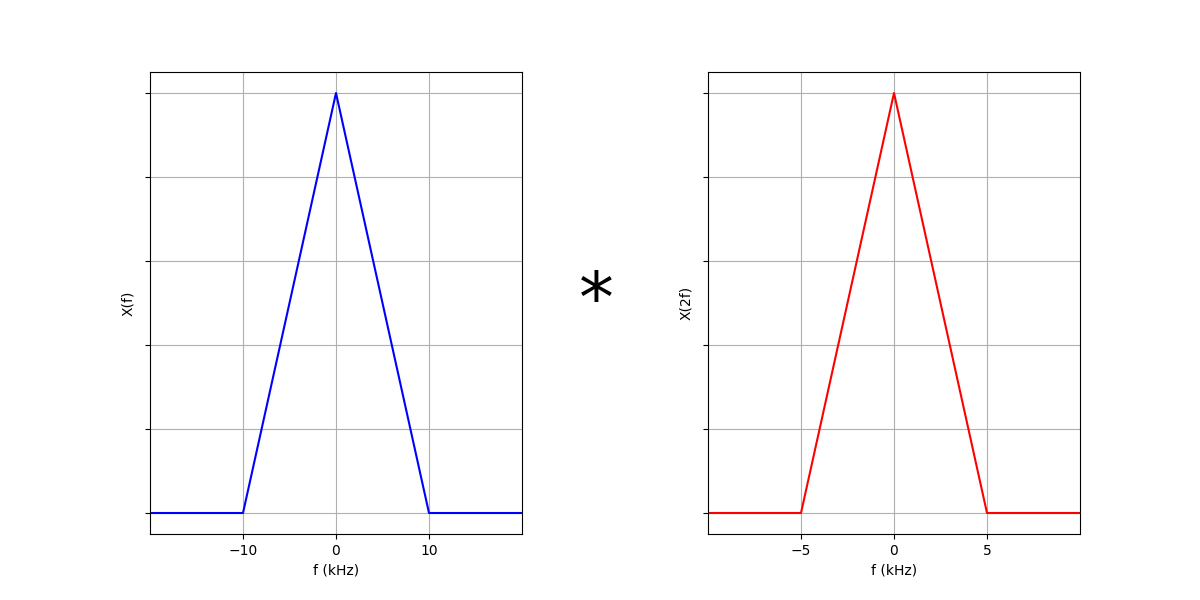
\includegraphics[width=\columnwidth]{figs/plot1.png}
    \caption{Plot of $X(f)$ and $X(2f)$}
    \label{fig:gate2021ec4fig1}
\end{figure}
\begin{figure}[h!]
    \centering
    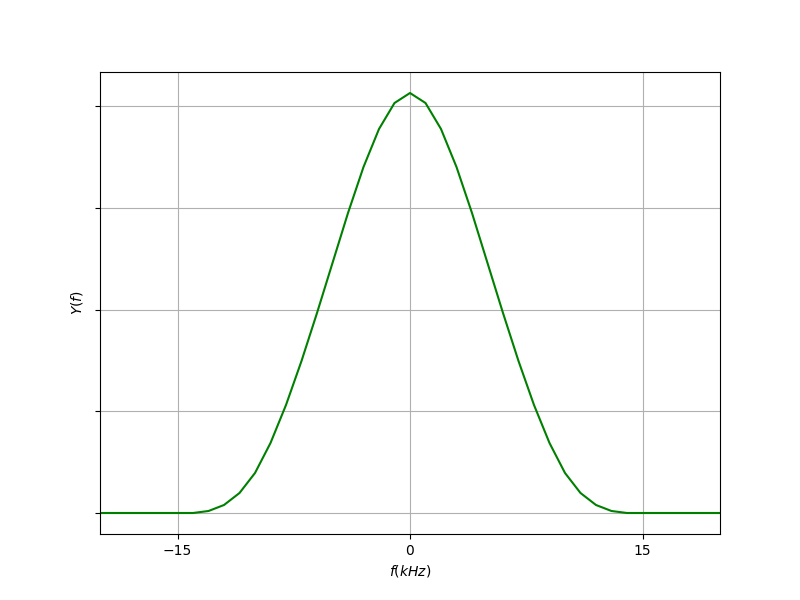
\includegraphics[width=\columnwidth]{figs/plot2.png}
    \caption{Plot of $Y(f)$}
    \label{fig:gate2021ec4fig2}
\end{figure}
Nyquist rate is $2f_{max} = 2(15kHz)$ which is $30kHz$
\end{document}

